\documentclass[a4paper, 11pt]{article}
\usepackage[a4paper, inner=3cm, outer=3cm, top=2cm, bottom=3cm]{geometry}
\usepackage{amsmath,calrsfs}
\usepackage{amsfonts}
\usepackage{tikz}




\begin{document}
	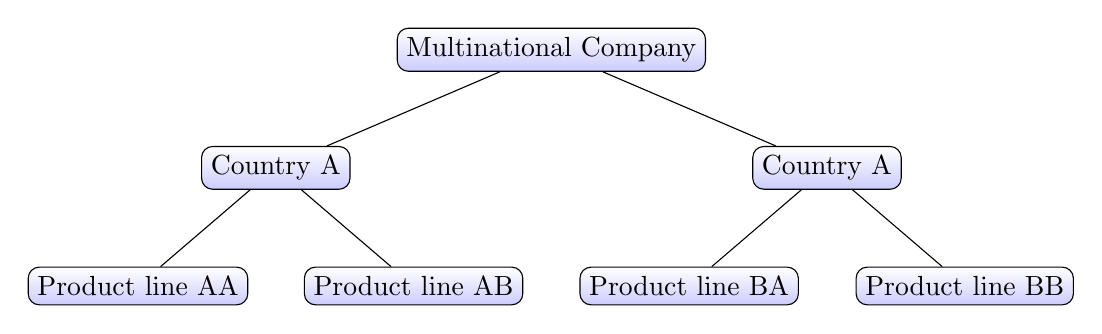
\begin{tikzpicture}[level/.style={sibling distance = 7cm/#1}, 
	every node/.style = {shape=rectangle, rounded corners,
		draw, align=center,
		top color=white, bottom color=blue!20}] 
	\node {Multinational Company}
	child{ node {Country A} 
			child{ node {Product line AA} }
			child{ node {Product line AB} }                            
		 }
	child{ node {Country A}
			child{ node {Product line BA} }
			child{ node {Product line BB} }
		 };
	  
	\end{tikzpicture}
	
	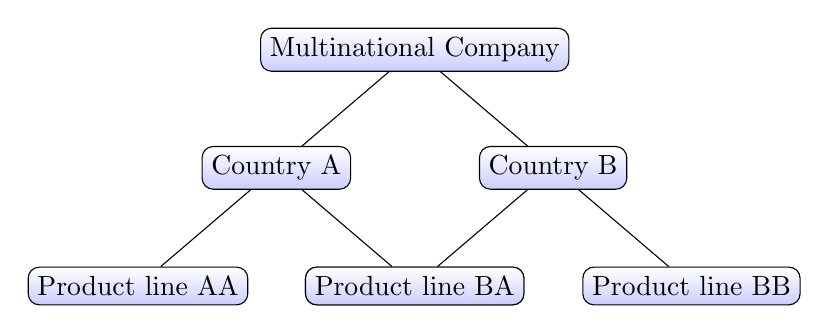
\begin{tikzpicture}[sibling distance=10em,
	every node/.style = {shape=rectangle, rounded corners,
		draw, align=center,
		top color=white, bottom color=blue!20}]
	\node {Multinational Company}
	child {node {Country A} 
			child {node {Product line AA}}
			child {node {Product line AB}}
		  }
	child {node {Country B} 
			child {node {Product line BA}}
			child {node {Product line BB}}
		  };
	\end{tikzpicture}
	
\end{document}